\section{Metodologia}\label{sec-metodologia}

O trabalho consiste em um estudo cienciométrico, de cunho descritivo e
abordagem quantitativa. Segundo \textcite{Macias-chapula1998} ``a cienciometria
é o estudo dos aspectos quantitativos da ciência''. Neste contexto,
\textcite{spinak1998} aponta que a cienciometria possibilita não apenas mapear
os trabalhos desenvolvidos na temática estudada, mas também verificar
tendências, lacunas e necessidades de estudo, além de propiciar a
compreensão da dispersão e da caducidade da produção do conhecimento.

A Biblioteca Brasileira de Dissertações e Teses foi a base de dados
utilizada. Os de busca foram os termos ``tecnologias digitais'' e
``PROEJA'', sendo \emph{AND} o operador \emph{booleano} utilizado. A
busca por estes descritores, resultou em 14 trabalhos. Pesquisou-se
igualmente com a combinação dos termos ``tecnologias digitais''
\emph{AND} ``educação profissional'' \emph{AND} ``jovens e adultos'',
tendo apenas 4 trabalhos retornantes e a busca pelos termos ``Tecnologia
digital da informação e comunicação'' \emph{AND} ``PROEJA'', a qual
retornou 1 trabalho. Foram critérios de inclusão, estarem disponíveis
para análise e terem como foco o estudo sobre o uso das tecnologias
digitais para o público de jovens e adultos da Educação Profissional.
Como o número de trabalhos retornantes era pequeno, não se realizou
nenhum recorte temporal. Após a leitura dos títulos e resumos, nove
trabalhos foram selecionados e analisados de acordo com a matriz
analítica apresentada na \Cref{fig1}.


\begin{figure}[htpb]
\centering
\begin{minipage}{.5\textwidth}
\caption{Matriz analítica utilizada para categorização dos trabalhos.}\label{fig1}
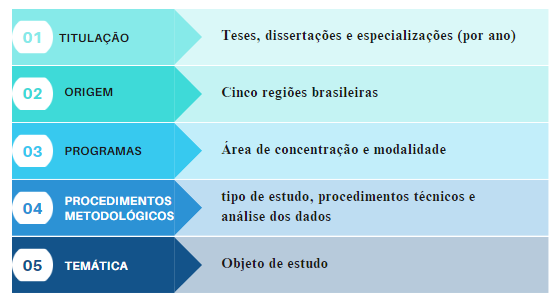
\includegraphics[width=\textwidth]{Fig1.png}
\source{as autoras}
\end{minipage}
\end{figure}


Os resultados da análise, segundo a matriz citada na \Cref{fig1}, são
descritos a seguir.